\documentclass[10pt,a4paper]{article}

% ===============================================================================
% PREAMBLE & PACKAGES
% ===============================================================================
\usepackage{fontspec}
\setmainfont{Latin Modern Roman}
\setmonofont{Latin Modern Mono}
\usepackage{unicode-math}
\setmathfont{Latin Modern Math}

\usepackage[margin=0.7in,top=0.9in,bottom=0.9in]{geometry}
\usepackage{xcolor}
\usepackage{tikz}
\usetikzlibrary{shapes.geometric, arrows.meta, positioning, calc, fit, decorations.pathreplacing}
\usepackage[most]{tcolorbox}
\usepackage{tabularx}
\usepackage{array}
\usepackage{enumitem}
\usepackage{amsmath}
\usepackage{fancyhdr}
\usepackage{microtype}
\usepackage[colorlinks=true,linkcolor=myteal,citecolor=mypurple,urlcolor=myblue]{hyperref}

\hyphenpenalty=10000
\exhyphenpenalty=10000
\sloppy

% ===============================================================================
% COLOR PALETTE (Strict adherence to spec)
% ===============================================================================
\definecolor{myred}{RGB}{196,30,58}       % section headings
\definecolor{mydark}{RGB}{30,30,50}       % body text
\definecolor{mygreen}{RGB}{14,120,80}     % definition boxes
\definecolor{myteal}{RGB}{0,130,140}      % formula boxes, diagrams, subsection headings
\definecolor{myamber}{RGB}{180,100,0}     % example boxes
\definecolor{mypurple}{RGB}{100,30,160}   % exam/viva boxes
\definecolor{myblue}{RGB}{25,90,170}      % hyperlinks/diagrams
\definecolor{mygray}{RGB}{246,247,249}    % tikzbox background
\definecolor{mgframe}{RGB}{180,185,200}   % tikzbox border
\definecolor{watermark}{RGB}{145,150,170} % footer watermark

\definecolor{hdrred}{RGB}{250,232,235}
\definecolor{hdrgreen}{RGB}{220,244,233}
\definecolor{hdrteal}{RGB}{220,242,244}
\definecolor{hdramber}{RGB}{253,242,215}
\definecolor{hdrpurple}{RGB}{238,228,255}
\definecolor{hdrblue}{RGB}{235,242,250}

% ===============================================================================
% TCOLORBOX STYLES
% ===============================================================================
\tcbset{
  tikzbox/.style={colback=mygray, colframe=mgframe, boxrule=0.6pt, arc=4pt,
    left=8pt, right=8pt, top=6pt, bottom=6pt,
    colbacktitle=mgframe, coltitle=mydark, fonttitle=\small\bfseries},
  defbox/.style={colback=hdrgreen, colframe=mygreen, boxrule=0.8pt, arc=4pt,
    left=9pt, right=9pt, top=6pt, bottom=6pt,
    colbacktitle=mygreen, coltitle=white, fonttitle=\small\bfseries},
  formulabox/.style={colback=hdrteal, colframe=myteal, boxrule=0.8pt, arc=4pt,
    left=9pt, right=9pt, top=7pt, bottom=7pt,
    colbacktitle=myteal, coltitle=white, fonttitle=\small\bfseries},
  examplebox/.style={colback=hdramber, colframe=myamber, boxrule=0.8pt, arc=4pt,
    left=9pt, right=9pt, top=6pt, bottom=6pt,
    colbacktitle=myamber, coltitle=white, fonttitle=\small\bfseries},
  masonbox/.style={colback=hdrpurple, colframe=mypurple, boxrule=0.8pt, arc=4pt,
    left=9pt, right=9pt, top=6pt, bottom=6pt,
    colbacktitle=mypurple, coltitle=white, fonttitle=\small\bfseries},
  exambox/.style={colback=hdrpurple, colframe=mypurple, boxrule=1pt, arc=5pt,
    left=10pt, right=10pt, top=8pt, bottom=8pt,
    colbacktitle=mypurple, coltitle=white, fonttitle=\bfseries,
    title after break={\textbf{Frequently Asked / Viva Questions (contd.)}}}
}
\tcbset{breakable}

% ===============================================================================
% TIKZ STYLES
% ===============================================================================
\tikzset{
  block/.style={rectangle, draw=myteal, fill=hdrteal, text width=2.4cm, align=center, minimum height=0.95cm, font=\small, rounded corners=3pt, line width=0.7pt},
  arrow/.style={-Stealth, thick, color=mydark},
  line/.style={thick, color=mydark}
}

% ===============================================================================
% MACROS & COMMANDS
% ===============================================================================
\newcommand{\Q}[1]{\textbf{#1}\par\vspace{2pt}}
\newcolumntype{Y}{>{\raggedright\arraybackslash}X}
\newcolumntype{C}{>{\centering\arraybackslash}X}

% Header & Footer
\pagestyle{fancy}
\fancyhf{}
\fancyhead[L]{\small\color{mydark}\textbf{OE-EC804B} --- Microwave Integrated Circuits}
\fancyhead[R]{\small\color{myteal}\textbf{Module 5 Notes}}
\fancyfoot[C]{\small\color{mydark}\thepage}
\fancyfoot[R]{\small\color{watermark}\copyright\ Biraj Sarkar}
\renewcommand{\headrulewidth}{0.6pt}

\hypersetup{pdftitle={OE-EC804B Module 5 Exam Notes}}

\begin{document}

% ===============================================================================
% TITLE BLOCK
% ===============================================================================
\begin{center}
  {\LARGE\bfseries\color{myred} OE-EC804B --- Microwave Integrated Circuits}\\[5pt]
  {\normalsize\color{mydark} Semester VIII \quad$\bullet$\quad 3L:0T:0P \quad$\bullet$\quad 3 Credits}\\[3pt]
  {\normalsize\color{myteal}\textbf{Module 5 Exam Notes: MIC Measurement, Testing \& Applications}}\\[3pt]
  {\small\color{mydark} CGEC \;$|$\; B.Tech ECE (2023--27) \;$|$\; \textit{Biraj Sarkar}}
\end{center}
\vspace{2pt}
\noindent{\color{myred}\rule{\linewidth}{1.5pt}}
\vspace{2pt}

\hypersetup{linkcolor=mydark}
\tableofcontents
\hypersetup{linkcolor=myteal}
\newpage

% ===============================================================================
% 1. MIC MEASUREMENT SYSTEMS, FIXTURES AND PROBES
% ===============================================================================
\section{MIC Measurement Systems, Fixtures and Probes}

Testing unpackaged MIC/MMIC chips presents unique challenges because standard coaxial cables (SMA, $2.92\text{ mm}$, $1.85\text{ mm}$) cannot interface directly with sub-millimeter planar microstrip pads on semiconductor wafers.

\begin{tcolorbox}[defbox, title={Microwave Test Fixture \& On-Wafer Probes}]
  A \textbf{Microwave Test Fixture} holds packaged or unpackaged MIC substrates and provides low-reflection transitions from coaxial launchers to planar microstrip traces. \textbf{On-Wafer RF Probes} (Ground-Signal-Ground / GSG coplanar probes) make direct electrical contact with MMIC pads on the semiconductor wafer using precision micro-positioning manipulators, operating up to $110\text{ GHz}$.
\end{tcolorbox}

\subsection{Wafer Probe Architecture (GSG Configuration)}
Coplanar GSG probes maintain a continuous $50\text{ }\Omega$ coplanar transmission line right up to the beryllium-copper or tungsten probe tips, completely eliminating wire bond series inductance ($L_s \approx 0$) during wafer-level characterization.

% ===============================================================================
% 2. S-PARAMETER MEASUREMENT AND CALIBRATION
% ===============================================================================
\section{S-Parameter Measurement and Calibration}

\subsection{Vector Network Analyzer (VNA)}
A \textbf{Vector Network Analyzer (VNA)} measures both the magnitude and phase of 2-port scattering parameters ($S_{11}, S_{21}, S_{12}, S_{22}$) by transmitting a frequency-swept RF signal and separating incident, reflected, and transmitted waves using internal directional couplers and heterodyne receivers.

\subsection{VNA Calibration \& Systematic De-Embedding}
Uncalibrated VNA measurements include systematic errors caused by cable attenuation, connector reflections, directional coupler directivity limits, and receiver frequency response. Calibration establishes mathematical error models to de-embed the fixture and move the measurement reference plane to the device under test (DUT).

\begin{enumerate}[leftmargin=*, itemsep=5pt]
  \item \textbf{SOLT Calibration (Short-Open-Load-Thru):}
    \begin{itemize}[leftmargin=*, noitemsep]
      \item Standard calibration for coaxial measurements using 4 known standards: Short ($\Gamma = -1$), Open ($\Gamma = +1$), Matched Load ($\Gamma = 0$), and Thru line ($S_{21} = 1$).
      \item \textit{Limitation in MMIC Testing:} Fabricating a precise, broadband $50\text{ }\Omega$ matched load standard on a semiconductor substrate is extremely difficult due to parasitic capacitance.
    \end{itemize}
  \item \textbf{TRL Calibration (Thru-Reflect-Line):}
    \begin{itemize}[leftmargin=*, noitemsep]
      \item Uses 3 simple planar standards printed directly on the substrate: a \textbf{Thru} line ($0$ length), an unknown high-reflection \textbf{Reflect} standard (Short or Open with identical $|\Gamma| \approx 1$), and a \textbf{Line} standard ($\lambda_g/4$ longer than Thru).
      \item \textbf{Primary calibration method for MMIC wafer probing} because it does not require a $50\text{ }\Omega$ matched load standard.
    \end{itemize}
\end{enumerate}

\begin{tcolorbox}[tikzbox, title={Vector Network Analyzer (VNA) S-Parameter Measurement Setup}]
\centering
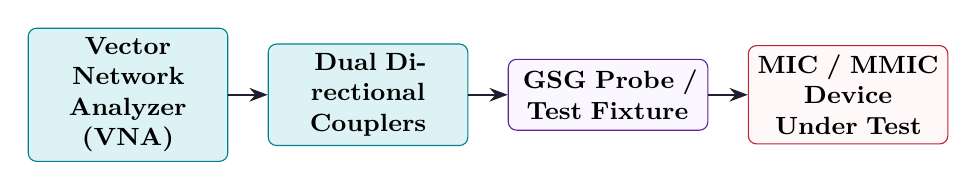
\begin{tikzpicture}[
  node distance=0.5cm, auto,
  sblock/.style={draw=myteal, fill=hdrteal, rectangle, rounded corners=3pt, align=center, font=\small\bfseries, minimum height=0.9cm, text width=2.3cm}
]
  \node [sblock] (vna) {Vector Network\\Analyzer (VNA)};
  \node [sblock, right=0.5cm of vna] (coupler) {Dual Directional\\Couplers};
  \node [sblock, fill=hdrpurple!30, draw=mypurple, right=0.5cm of coupler] (probe) {GSG Probe /\\Test Fixture};
  \node [sblock, fill=hdrred!30, draw=myred, right=0.5cm of probe] (dut) {MIC / MMIC\\Device Under Test};

  \draw [arrow] (vna) -- (coupler);
  \draw [arrow] (coupler) -- (probe);
  \draw [arrow] (probe) -- (dut);
\end{tikzpicture}
\end{tcolorbox}

% ===============================================================================
% 3. NOISE MEASUREMENT TECHNIQUES
% ===============================================================================
\section{Noise Figure Measurement Techniques}

Noise Figure ($NF$) measures the degradation of Signal-to-Noise Ratio (SNR) as a signal passes through a microwave circuit:
\begin{equation}
  F = \frac{\text{SNR}_{in}}{\text{SNR}_{out}} \quad ; \quad NF (\text{dB}) = 10 \log_{10}(F)
\end{equation}

\subsection{The Y-Factor Measurement Method}
The \textbf{Y-Factor Method} is the industry standard technique for measuring Noise Figure using a calibrated noise source toggled between two known noise temperatures: \textbf{HOT ($T_H$)} and \textbf{COLD ($T_C$)}.

\begin{tcolorbox}[formulabox, title={Y-Factor Derivation \& Noise Figure Equations}]
  Noise power measured at receiver output for HOT and COLD states:
  \begin{equation}
    N_{\text{HOT}} = k (T_H + T_e) B \cdot G \quad ; \quad N_{\text{COLD}} = k (T_C + T_e) B \cdot G
  \end{equation}
  Taking the ratio yields the dimensionless $Y$-factor:
  \begin{equation}
    Y = \frac{N_{\text{HOT}}}{N_{\text{COLD}}} = \frac{T_H + T_e}{T_C + T_e} \implies T_e = \frac{T_H - Y T_C}{Y - 1}
  \end{equation}
  The noise factor $F$ relative to reference temperature $T_0 = 290\text{ K}$ ($27^\circ\text{C}$):
  \begin{equation}
    F = 1 + \frac{T_e}{T_0} = \frac{\text{ENR}}{Y - 1} \quad \text{where } \text{ENR} = \frac{T_H - T_0}{T_0} \text{ (Excess Noise Ratio)}
  \end{equation}
\end{tcolorbox}

\begin{tcolorbox}[examplebox, title={Worked Numerical: Noise Figure Calculation via Y-Factor Method}]
  \textbf{Problem:} A noise source with an Excess Noise Ratio $\text{ENR} = 15.0\text{ dB}$ is connected to a microwave amplifier. The measured output noise power ratio between HOT and COLD states is $Y = 8.0\text{ dB}$. Calculate:
  \begin{enumerate}[label=(\alph*), noitemsep]
    \item The linear ENR and linear $Y$-factor.
    \item The Noise Factor $F$ and Noise Figure $NF$ in dB.
  \end{enumerate}
  \tcblower
  \textbf{Solution:}
  \begin{enumerate}[label=(\alph*), itemsep=4pt]
    \item Convert values from dB to linear ratios:
      \begin{equation}
        \text{ENR}_{\text{linear}} = 10^{15/10} = 10^{1.5} = 31.6228
      \end{equation}
      \begin{equation}
        Y_{\text{linear}} = 10^{8/10} = 10^{0.8} = 6.30957
      \end{equation}
    \item Calculate Noise Factor $F$:
      \begin{equation}
        \begin{aligned}
          F &= \frac{\text{ENR}_{\text{linear}}}{Y_{\text{linear}} - 1} = \frac{31.6228}{6.30957 - 1} \\
          &= \frac{31.6228}{5.30957} = 5.9558
        \end{aligned}
      \end{equation}
      Convert $F$ to Noise Figure $NF$ in dB:
      \begin{equation}
        NF = 10 \log_{10}(5.9558) = 7.749\text{ dB} \approx 7.75\text{ dB}
      \end{equation}
  \end{enumerate}
\end{tcolorbox}

% ===============================================================================
% QUICK REVISION PAGE
% ===============================================================================
\newpage
\begin{center}
  {\large\bfseries\color{myred} Quick Revision --- Module 5}\\[3pt]
  {\small\color{mydark} MIC Measurement, Testing \& Applications $|$ OE-EC804B}
\end{center}
\noindent{\color{myred}\rule{\linewidth}{1.2pt}}
\vspace{4pt}

\begin{tcolorbox}[formulabox, title={\textbf{Key Concepts and Metrics at a Glance}}]
\renewcommand{\arraystretch}{1.35}
\begin{tabularx}{\linewidth}{>{\raggedright\arraybackslash\bfseries}p{4.5cm} X}
Vector Network Analyzer (VNA) & Measures magnitude \& phase of 2-port S-parameters ($S_{11}, S_{21}, S_{12}, S_{22}$). \\[4pt]
TRL Calibration & Thru-Reflect-Line method; preferred for MMIC wafer probes as no matched load standard is required. \\[4pt]
GSG Wafer Probes & Ground-Signal-Ground coplanar probes providing $50\text{ }\Omega$ contact directly to MMIC pads. \\[4pt]
Y-Factor Noise Measurement & Toggles noise source between HOT ($T_H$) and COLD ($T_C$) states ($Y = N_{\text{HOT}}/N_{\text{COLD}}$). \\[4pt]
Excess Noise Ratio (ENR) & $\text{ENR} = (T_H - T_0)/T_0$; specifies calibrated output power of RF noise head. \\
\end{tabularx}
\end{tcolorbox}

\begin{tcolorbox}[defbox, title={\textbf{One-Line Definitions}}]
  \begin{itemize}[leftmargin=*, noitemsep]
    \item \textbf{VNA:} Microwave instrument measuring complex reflection and transmission parameters of RF networks.
    \item \textbf{GSG Probe:} High-frequency coplanar probe contacting MMIC wafer pads without wire bond inductance.
    \item \textbf{TRL Calibration:} De-embedding calibration technique utilizing Thru, Reflect, and Line standards on substrate.
    \item \textbf{Y-Factor Method:} Standard microwave technique for measuring Noise Figure via hot/cold noise ratio.
  \end{itemize}
\end{tcolorbox}

\begin{tcolorbox}[exambox, title={\textbf{Frequently Asked / Viva Questions}}]
  \begin{enumerate}[topsep=0pt, label=\textbf{Q\arabic*.}, itemsep=5pt]
    \item \Q{What is the function of a Vector Network Analyzer (VNA)?}
    A VNA measures the complex scattering parameters ($S$-parameters: magnitude and phase) of microwave components over a swept frequency range.

    \item \Q{Why is calibration required before performing VNA measurements?}
    Calibration removes systematic errors introduced by test cables, connectors, attenuators, and internal VNA directional couplers.

    \item \Q{Differentiate between SOLT and TRL calibration.}
    SOLT uses Short, Open, Load, and Thru coaxial standards. TRL uses Thru, Reflect, and Line planar standards and is preferred for MMIC on-wafer probing because it does not require a $50\text{ }\Omega$ matched load standard.

    \item \Q{What is an On-Wafer GSG Probe?}
    A Ground-Signal-Ground coplanar RF probe that makes direct electrical contact with MMIC pads on the semiconductor wafer up to $110\text{ GHz}$.

    \item \Q{Explain the Y-Factor method for Noise Figure measurement.}
    The Y-Factor method measures output noise power when a noise source is switched HOT ($T_H$) and COLD ($T_C$). The ratio $Y = N_{\text{HOT}}/N_{\text{COLD}}$ determines effective noise temperature $T_e$ and Noise Figure $NF$.

    \item \Q{Define Excess Noise Ratio (ENR) of a noise source.}
    $\text{ENR} = (T_H - T_0)/T_0$, expressed in dB. It quantifies the calibrated noise power output above standard room temperature ($T_0 = 290\text{ K}$).

    \item \Q{What is a microwave test fixture?}
    A mechanical housing that holds an unencapsulated MIC substrate and provides low-reflection transitions between coaxial cables and planar microstrip lines.

    \item \Q{What is reference plane shift in S-parameter measurements?}
    The mathematical offset applied by VNA calibration to move the measurement plane from the coaxial cable tips directly to the MIC substrate ports.

    \item \Q{Why is Noise Figure measurement sensitive to receiver gain?}
    High receiver gain prevents internal meter noise from masking the small noise power differences ($N_{\text{HOT}} - N_{\text{COLD}}$) generated by the Device Under Test.

    \item \Q{What is the role of de-embedding in MIC testing?}
    De-embedding mathematically subtracts the known parasitic $S$-parameters of test fixtures and launches from the measured data to isolate the intrinsic MIC device response.
  \end{enumerate}
\end{tcolorbox}

\end{document}
